\documentclass[letterpaper]{article}
\usepackage[margin=1in]{geometry}
\usepackage[utf8]{inputenc}
\usepackage{textcomp}
\usepackage{amssymb}
\usepackage{natbib}
\usepackage{graphicx}
\usepackage{gensymb}
\usepackage{amsthm, amsmath, mathtools}
\usepackage[dvipsnames]{xcolor}
\usepackage{enumerate}
\usepackage{mdframed}
\usepackage[most]{tcolorbox}
\usepackage{csquotes}
% https://tex.stackexchange.com/questions/13506/how-to-continue-the-framed-text-box-on-multiple-pages

\tcbuselibrary{theorems}

\newcommand{\R}{\mathbb{R}}
\newcommand{\Z}{\mathbb{Z}}
\newcommand{\N}{\mathbb{N}}
\newcommand{\Q}{\mathbb{Q}}
\newcommand{\C}{\mathbb{C}}
\newcommand{\code}[1]{\texttt{#1}}
\newcommand{\mdiamond}{$\diamondsuit$}
\newcommand{\PowerSet}{\mathcal{P}}
\newcommand{\Mod}[1]{\ (\mathrm{mod}\ #1)}
\DeclareMathOperator{\lcm}{lcm}

%\newtheorem*{theorem}{Theorem}
%\newtheorem*{definition}{Definition}
%\newtheorem*{corollary}{Corollary}
%\newtheorem*{lemma}{Lemma}
\newtheorem*{proposition}{Proposition}


\newtcbtheorem[number within=section]{theorem}{Theorem}
{colback=green!5,colframe=green!35!black,fonttitle=\bfseries}{th}

\newtcbtheorem[number within=section]{definition}{Definition}
{colback=blue!5,colframe=blue!35!black,fonttitle=\bfseries}{def}

\newtcbtheorem[number within=section]{corollary}{Corollary}
{colback=yellow!5,colframe=yellow!35!black,fonttitle=\bfseries}{cor}

\newtcbtheorem[number within=section]{lemma}{Lemma}
{colback=red!5,colframe=red!35!black,fonttitle=\bfseries}{lem}

\newtcbtheorem[number within=section]{example}{Example}
{colback=white!5,colframe=white!35!black,fonttitle=\bfseries}{def}

\newtcbtheorem[number within=section]{note}{Important Note}{
        enhanced,
        sharp corners,
        attach boxed title to top left={
            xshift=-1mm,
            yshift=-5mm,
            yshifttext=-1mm
        },
        top=1.5em,
        colback=white,
        colframe=black,
        fonttitle=\bfseries,
        boxed title style={
            sharp corners,
            size=small,
            colback=red!75!black,
            colframe=red!75!black,
        } 
    }{impnote}
\usepackage[utf8]{inputenc}
\usepackage[english]{babel}
\usepackage{fancyhdr}
\usepackage[hidelinks]{hyperref}

\pagestyle{fancy}
\fancyhf{}
\rhead{MATH 155A}
\chead{Thursday, March 31, 2022}
\lhead{Lecture 2}
\rfoot{\thepage}

\setlength{\parindent}{0pt}

\begin{document}

\section{Introduction to Shader Programs}
We'll begin by showing the process behind drawing a triangle. Consider the following triangle:
\begin{center}
    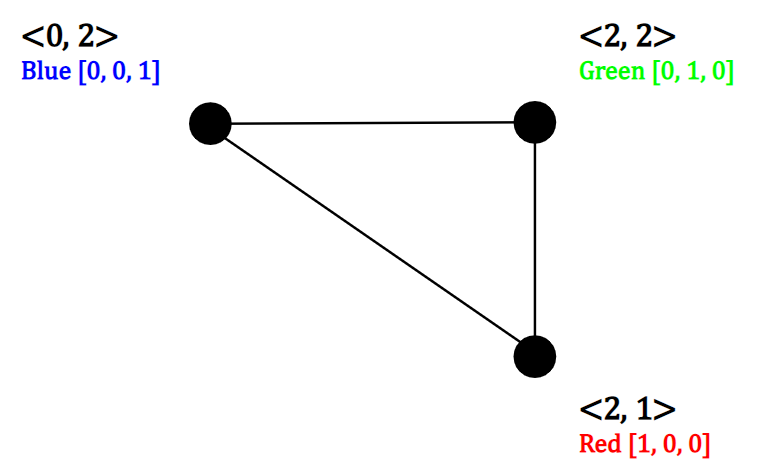
\includegraphics[scale=0.6]{../assets/shader1.png}
\end{center}
Here, we want to make the vertex at: 
\begin{itemize}
    \item $\cyclic{2, 1}$ red. We'll call this vertex $R$.
    \item $\cyclic{2, 2}$ green. We'll call this vertex $G$.
    \item $\cyclic{0, 2}$ blue. We'll call this vertex $B$. 
\end{itemize}
Note that the tuple next to the color, $[R, G, B]$, is the RGB color specification. Then, when we actually draw this triangle, the color at any particular point will just be the averages of the other base colors. For examples:
\begin{itemize}
    \item The vertex directly in the center (the midpoint) of $B$ and $R$ would have the averages of the two RGB values of the two vertices; in other words, at that particular point, we would have the RGB value $\cyclic{\frac{1}{2}, 0, \frac{1}{2}}$ (dark magenta).
    \item The vertex directly in the center (the midpoint) of $B$ and $G$ would have the RGB value $\cyclic{0, \frac{1}{2}, \frac{1}{2}}$ (cyan).
    \item The vertex directly in the center of $G$ and $R$ would have the RGB value $\cyclic{\frac{1}{2}, \frac{1}{2}, 0}$ (yellow). 
    \item The vertex directly in the center of all three vertices $R$, $G$, and $B$ (i.e. at the center of the triangle) would have the RGB value $\cyclic{\frac{1}{3}, \frac{1}{3}, \frac{1}{3}}$ (gray). 
\end{itemize}

We'll now see how the corresponding C++ code works. 
\begin{enumerate}
    \item Build a C++ array of vertex attributes\footnote{Numeric properties of the vertex.}. That is, the position and color.
    \begin{verbatim}
        float verts[] = {
            2, 1, // bottom-right vertex position; point (2, 1) 
            1, 0, 0, // color of vertex at (2, 1) 
            2, 2, // top-right vertex position; point (2, 2)
            0, 1, 0, // color of vertex at (2, 2)
            0, 2, // top-left vertex position; point (0, 2)
            0, 0, 1 // color of vertex at (0, 2)
        };\end{verbatim}
    
    \item We now load the data from the C++ array into the OpenGL buffers on the GPU. We'll just explain a subset of the commands due to there being many commands.  
    \begin{verbatim}
        glBufferData(GL_BUFFER_ARRAY, sizeof(verts), verts, GL_STATIC_DRAW);\end{verbatim}
    What \code{glBufferData} does is it loads the C++ array into the OpenGL buffer. The parameters are as follows: 
    \begin{itemize}
        \item \code{GL\_BUFFER\_ARRAY}: This tells the program where to send the data to. This is sometimes called the Vertex Buffer Object. 
        \item \code{sizeof(verts)}: The amount of data to send, in bytes.
        \item \code{verts}: The data to send. This starts from the beginning of the array and sends \code{sizeof(verts)} data (the previous parameter).
        \item \code{GL\_STATIC\_DRAW}: A ``hint'' telling OpenGL how your data should be used. Here, we're saying that this is some fixed data that we won't be changing much. 
    \end{itemize}
    All we did was send a bunch of data to the buffer. We now need to tell OpenGL what the data is. 
    \begin{verbatim}
    glVertexAttribPointer(0, 2, GL_FLOAT, GL_FALSE, 5 * sizeof(float), (void*) 0);\end{verbatim}
    This command tells OpenGL \emph{what exactly} we sent. The parameters are: 
    \begin{itemize}
        \item \code{0}: The location which holds the $xy$ coordinates. 
        \item \code{2}: The number of data items that are a part of this location. In this particular example, this is $x$ and $y$.
        \item \code{GL\_FLOAT}: We're adding floating point numbers. Pairing this with the previous parameters, this means that we're adding two floating point numbers. 
        \item \code{5 * sizeof(float)}: The stride, or the \emph{step}. In this case, we're essentially saying that 
        \[\{\underbrace{2, 1, 1, 0, 0}_{\text{Stride}}, \underbrace{2, 2, 0, 1, 0}_{\text{Stride}}, \underbrace{0, 2, 0, 0, 1}_{\text{Stride}}\}\]
        Put it another way, we're just telling OpenGL what set of data represents a vertex.
        \item  \code{(void*) 0}: The starting position, or the first $xy$.
    \end{itemize}
    Now, we need to turn this on. So, we have the command: 
    \begin{verbatim}
        glEnableVertexAttribArray(0);
    \end{verbatim}
    So, the previous command tells OpenGL where the data starts. This command tells OpenGL to use that data at the specified location (the parameter). Here, the parameter is: 
    \begin{itemize}
        \item \code{0}: Location 0. In other words, this parameter is the same value as the first parameter in the previous command. This tells OpenGL to use the data at location 0.
    \end{itemize}

    Note that the above was for $xy$ values. How would we change this for the color values? In particular: 
    \begin{itemize}
        \item We now need to tell OpenGL what the data is. 
        \begin{verbatim}
glVertexAttribPointer(1, 3, GL_FLOAT, GL_FALSE, 5 * sizeof(float), (void*) 0);\end{verbatim}
        This command tells OpenGL \emph{what exactly} we sent. The parameters are: 
        \begin{itemize}
            \item \code{0}: The location which will hold the RGB values.
            \item \code{2}: The number of data items that are a part of this location. In this particular example, this is $x$ and $y$.
            \item \code{GL\_FLOAT}: We're adding floating point numbers. Pairing this with the previous parameters, this means that we're adding two floating point numbers. 
            \item \code{5 * sizeof(float)}: The stride, or the \emph{step}. In this case, we're essentially saying that 
            \[\{2, 1, \underbrace{1, 0, 0, 2, 2}_{\text{Stride}}, \underbrace{0, 1, 0, 0, 2}_{\text{Stride}}, 0, 0, 1\}\]
            Put it another way, we're just telling OpenGL what set of data represents the colors.
            \item  \code{(void*) 2 * sizeof(float)}: The starting position, or the position of the first set of RGB values.
        \end{itemize}
        Now, we need to turn this on. So, we have the command: 
        \begin{verbatim}
            glEnableVertexAttribArray(1);
        \end{verbatim}
        So, the previous command tells OpenGL where the data starts. This command tells OpenGL to use that data at the specified location (the parameter). Here, the parameter is: 
        \begin{itemize}
            \item \code{1}: Location 1. In other words, this parameter is the same value as the first parameter in the previous command. We're telling OpenGL to read the data from location 1.
        \end{itemize}
    \end{itemize}

    \item Compile and link the shadow programs. The shader program consists of two different types of shaders.
    \begin{itemize}
        \item \underline{Vertex Shader:} Runs on each vertex. 
        \begin{verbatim}
            // GLSL Version 
            #version 330 core     
            layout(location = 0) in vec3 vertPos;\end{verbatim}
        Here, this is saying that we have a variable \code{vertPos} which is a \code{vec3} (a vector of 3 floating point numbers), identified at location 0, which we described in the previous step. \code{vertPos} described the vertex's position. Note that, in the VBO, we only gave 2 values; thus, \code{z} will be set to 0.
        
        \begin{verbatim}
            layout (location = 1) in vec3 color;\end{verbatim}
        This is similar to the previous line of code, except that we're defining this for RGB values instead. 

        \begin{verbatim}
            out vec3 theColor;\end{verbatim}
        We're now outputting a \code{vec3} called \code{theColor}.

        \begin{verbatim}
            void main() {
                gl_Position = vec4(vertPos.x - 1, vertPos.y - 1, 0, 1);
            \end{verbatim}
        Here, we're outputting a vector with four components (it'll always be a \code{vec4}); an $x$, $y$, $z$, and $w$ component, respectively. Note that $x, y, z, w \in [-1, 1]$. The reason why we subtract 1 from the $x$, $y$ coordinates is because we have vertices whose $x$- and $y$-coordinates are in the range $[0, 2]$. 

        \begin{verbatim}
                theColor = color;
            } \end{verbatim}
        We just keep the color positions as is. This concludes this particular program; note that this program is executed once per vertex. 

        \item \underline{Fragment Shader:} This is run once for every pixel covered by the triangle. This is given by: 
        \begin{verbatim}
            // GLSL Version 
            #version 330 core
            in vec3 theColor; \end{verbatim}
        Here, the input \code{vec3} is given by the output \code{vec3}. 

        \begin{verbatim}
            out vec4 pixelColor;\end{verbatim}
        This defines the output color of the pixel. 

        \begin{verbatim}
            void main() {
                pixelColor = vec4(theColor, 1);
            }\end{verbatim}
        Here, the \code{1} indicates no transparency; this is sometimes known as the alpha value. 
    \end{itemize}
    

    \item Draw the triangle using a C++ command. 
    \begin{verbatim}
        glDrawArrays(GL_TRIANGLE, 0, 3);\end{verbatim}
    Here: 
    \begin{itemize}
        \item \code{0} means to start with vertex 0 in the array of data that was uploaded. 
        \item \code{3} means the number of vertices to process. 
    \end{itemize}
    This tells the shader program to render the triangle.  
\end{enumerate}



\end{document}